\section{TaskBatch}

\subsection{Código}

\begin{lstlisting}[language=C++, breaklines=true]
void TaskBatch(int pid, vector<int> params) {

	srand(1); // set seed

	int total_cpu = params[0];
	int cant_bloqueos = params[1];

	bool config[total_cpu];
	fill_n(config, total_cpu, false);
	for (int i = 0; i < cant_bloqueos; i++) config[i] = true;
	random_shuffle(&config[0], &config[total_cpu-1]);

	for (int i = 0; i < total_cpu; ++i) {
		if (config[i] == true) { // block
			uso_IO(pid, 1);
		} else {
			uso_CPU(pid, 1);
		}
	}
}
\end{lstlisting}

El codigo que simula la tarea \texttt{TaskBatch} recibe dos parametros, estos son la cantidad de total de ciclos de reloj que lleva ejecutar la tarea y la cantidad de llamadas bloqueantes que ocurriran durante la ejecucion de la misma. A partir de la cantidad total de ciclos de CPU, se arma un vector en donde van a estar colocados los momentos donde ocurra una llamada bloqueante, estos se colocan de manera pseudoaleatoria con la funcion \texttt{random\_shuffle}. Una vez que termine este proceso, procedemos a simular la ejecucion de los ciclos de CPU utilizando el vector, si este indica que se debe producir una llamada bloqueante hace una llamada a \texttt{uso\_IO}, en el caso contrario se ejecuta un ciclo de CPU.

\subsubsection{Diagrama GANTT}

El siguiente diagrama fue generado con los siguientes parametros:

\begin{enumerate}
	\item lote\_tsk: 3.tsk
	\item num\_cores: 1
	\item switch\_cost: 1
	\item sched\_class: SchedFCFS
\end{enumerate}

\begin{figure}[h]
    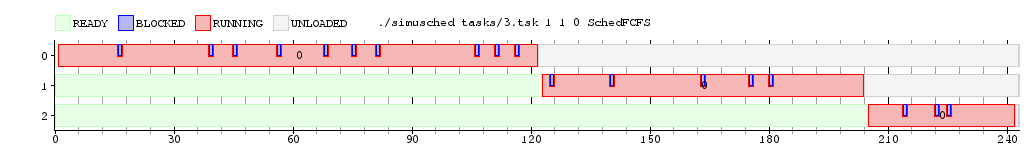
\includegraphics[width=\linewidth]{images/3.png}
    \label{fig:Task Consola}
    \caption{Task Batch}
\end{figure}

En la figura 4 tenemos el diagrama de Gantt de la ejecucion de tareas del lote 3, las tareas ejecutadas en el mismo cumplen con los siguientes parametros:

\begin{itemize}
	\item Tarea 0: 100 ciclos de CPU, 10 llamadas bloqueantes
	\item Tarea 1: 70 ciclos de CPU, 5 llamadas bloqueantes
	\item Tarea 2: 30 ciclos de CPU, 3 llamadas bloqueantes
\end{itemize}

Como podemos apreciar, el diagrama cumple perfectamente con el scheduler FCFS, es decir, las tareas no son desalojadas y se las mantiene en ejecucion hasta que concluyan. Ademas podemos ver que el diagrama respeta el costo de hacer una llamada bloqueante, tomando un ciclo adicional antes de efectuar las mismas.